%
% Jan Pribošek
% Diplomska naloga
%%%%%%%%%%%%%%%%%%%%%%%%%%%%%%%%%%%%%%%%%%%%%%%%%%%%%%%%%%%%%%%%%%%%%%%%%%%
\documentclass[11pt,a4paper,twoside,fleqn,openany]{book}
%%%%%%%%%%%%%%%%%%%%%%%%%%%%%%%%%%%%%%%%%%%%%%%%%%%%%%%%%%%%%%%%%%%%%%%%%%%

% Nastavitve strani
\setlength{\voffset}{-1 in}        % premakne koordinatno izhodisce strani na zg. rob lista
\setlength{\hoffset}{-1 in}        % premakne koordinatno izhodisce strani na levi. rob lista
\setlength{\oddsidemargin}{3 cm}   % velikost levega robu na sodih straneh
\setlength{\evensidemargin}{2 cm}  % velikost levega robu na lihih straneh
\setlength{\topmargin}{1.5 cm}     % velikost zgornjega robu do glave
\setlength{\headheight}{1 cm}      % velikost glave
\setlength{\headsep}{0.5 cm}       % glava od teksta
\setlength{\textwidth}{16 cm}      % sirina besedila
\setlength{\textheight}{24.7 cm}   % visina besedila
\setlength{\footskip}{1 cm}        % noga od teksta
\setlength{\marginparsep}{3 mm}    % ni vazno
\setlength{\marginparwidth}{0 cm}  % ni vazno
%
% Nastavitve odstavka
\setlength{\parindent}{0 mm}       % zamik prve vrstice odstavka
\setlength{\parskip}{1.5ex}        % razmik med odstavki
\renewcommand{\baselinestretch}{1.2}% razmik med vrsticami
\setlength{\mathindent}{1 cm}       % zamik ena?b od levega roba

\usepackage{times}
\usepackage[slovene]{babel}
\usepackage[utf8]{inputenc}
\usepackage[pdftex]{graphicx, color}

\usepackage{amsfonts}
\usepackage{amsmath}
\usepackage{nccmath}
\usepackage{tabularx}
\usepackage{mathptmx}
\usepackage{fancyhdr}
\usepackage{mathtools}
\usepackage{framed}
\usepackage{wasysym}			% paket ki omogoča oznako promil
\usepackage{booktabs}			% paket za tabele
%\usepackage[pdftex,unicode]{hyperref}
\usepackage[pdftex,unicode,colorlinks,linkcolor=blue,citecolor=blue,urlcolor=blue]{hyperref}
\urlstyle{same}

% enumerate with roman numerals
\usepackage{enumerate}
\usepackage[shortlabels]{enumitem}

\usepackage{cite}
\usepackage{pdfpages}
\usepackage{color}
\definecolor{mygray}{gray}{.6}

%\usepackage{lastpage}
%\usepackage{totcount}
%\regtotcounter{figure}
%\regtotcounter{page}
\usepackage[figure,table,page,equation]{totalcount}

\usepackage{float}
\usepackage{multirow}
\usepackage[center]{subfigure}
%\usepackage{natbib}

% Paket za prilagajanje napisov pod plavajočimi objekti
\usepackage[subfigure]{ccaption}
\captionstyle{\centering}

% customizing lists
\usepackage{enumitem}


% Urejanaje kazal
% Za osnovn kazala popravljam kar osnovno definicijo v book.cls
\AtBeginDocument{
\renewcommand\contentsname{KAZALO VSEBINE}
\renewcommand\listfigurename{KAZALO SLIK}
\renewcommand\listtablename{KAZALO PREGLEDNIC}
\renewcommand{\bibname}{VIRI}
\renewcommand\tablename{Preglednica}
}

%
% in seznam prilog
\usepackage[subfigure, titles]{tocloft} % Paket za nastavitev seznamov

% Seznam slik v ang. - removed 7.3
%\newcommand{\listfigname}{LIST OF FIGURES}
%\newlistof[chapter]{ffigure}{loff}{\listfigname}
% nov ukaz za dodajanje slik v seznam slik
%\newcommand{\addfiguretolof}[1]{
%\addcontentsline{loff}{figure}{\protect\numberline{\thefigure}#1}
%}
% Seznam preglednic v angl
%\newcommand{\listtabname}{LIST OF TABLES}
%\newlistof[chapter]{ttable}{lott}{\listtabname}
% nov ukaz za dodajanje preglednic v seznam preglednic
%\newcommand{\addtabletolot}[1]{
%\addcontentsline{lott}{figure}{\protect\numberline{\thetable}#1}
%}
% Seznam prilog
\newcommand{\listappname}{SEZNAM DODATKOV}
%\newlistof[chapter]{appendices}{loapp}{\listappname}
%\cftpagenumbersoff{appendices}
%\renewcommand{\cftappendicesdotsep}{\cftnodots}


%\usepackage{setspace}
%\onehalfspacing

%Nastavitve nasplovov/podnaslovov...
\usepackage{titlesec}

% solve bug in titlesec package (numbers on chapters are not showing)
\usepackage{etoolbox}
\makeatletter
\patchcmd{\ttlh@hang}{\parindent\z@}{\parindent\z@\leavevmode}{}{}
\patchcmd{\ttlh@hang}{\noindent}{}{}{}
\makeatother



\titleformat{\chapter}[hang]
{\normalfont\bfseries\normalsize}
{\thechapter}{2mm}{}
\titlespacing{\chapter}{0pt}{\baselineskip}{\baselineskip}


\titleformat{\section}[hang]
{\normalfont\bfseries\normalsize}
{\thesection}{2mm}{}

\titleformat{\subsection}[hang]
{\normalfont\bfseries\normalsize}
{\thesubsection}{2mm}{}


\SetSymbolFont{letters}{normal}{OML}{cmr}{m}{n}
\SetSymbolFont{letters}{bold}{OML}{cmm}{b}{it}
\SetSymbolFont{operators}{bold}{OT1}{cmr}{bx}{n}
%
\newcommand{\bs}[1]{\boldsymbol{#1}}
\newcommand{\bm}[1]{\mathbf{#1}}


\newcommand\bcdot{\ensuremath{%
  \mathchoice%
   {\mskip\thinmuskip\lower0.2ex\hbox{\scalebox{1.5}{$\cdot$}}\mskip\thinmuskip}}%
   {\mskip\thinmuskip\lower0.2ex\hbox{\scalebox{1.5}{$\cdot$}}\mskip\thinmuskip}%        
   {\lower0.3ex\hbox{\scalebox{1.2}{$\cdot$}}}%  
   {\lower0.3ex\hbox{\scalebox{1.2}{$\cdot$}}}%
}




\begin{document}

\allowdisplaybreaks[1]

%------------------------------------
% Naslovnica
%------------------------------------
\frontmatter
\thispagestyle{empty}

% content should be on the same page
\begin{minipage}{\textwidth}

\begin{center}
%\vspace*{-1.5 cm}
%\textsc{Univerza v Ljubljani}\\
%\textsc{Fakulteta za gradbeništvo in geodezijo}

\vspace*{-3cm}


\begin{center}
\advance\leftskip-2cm
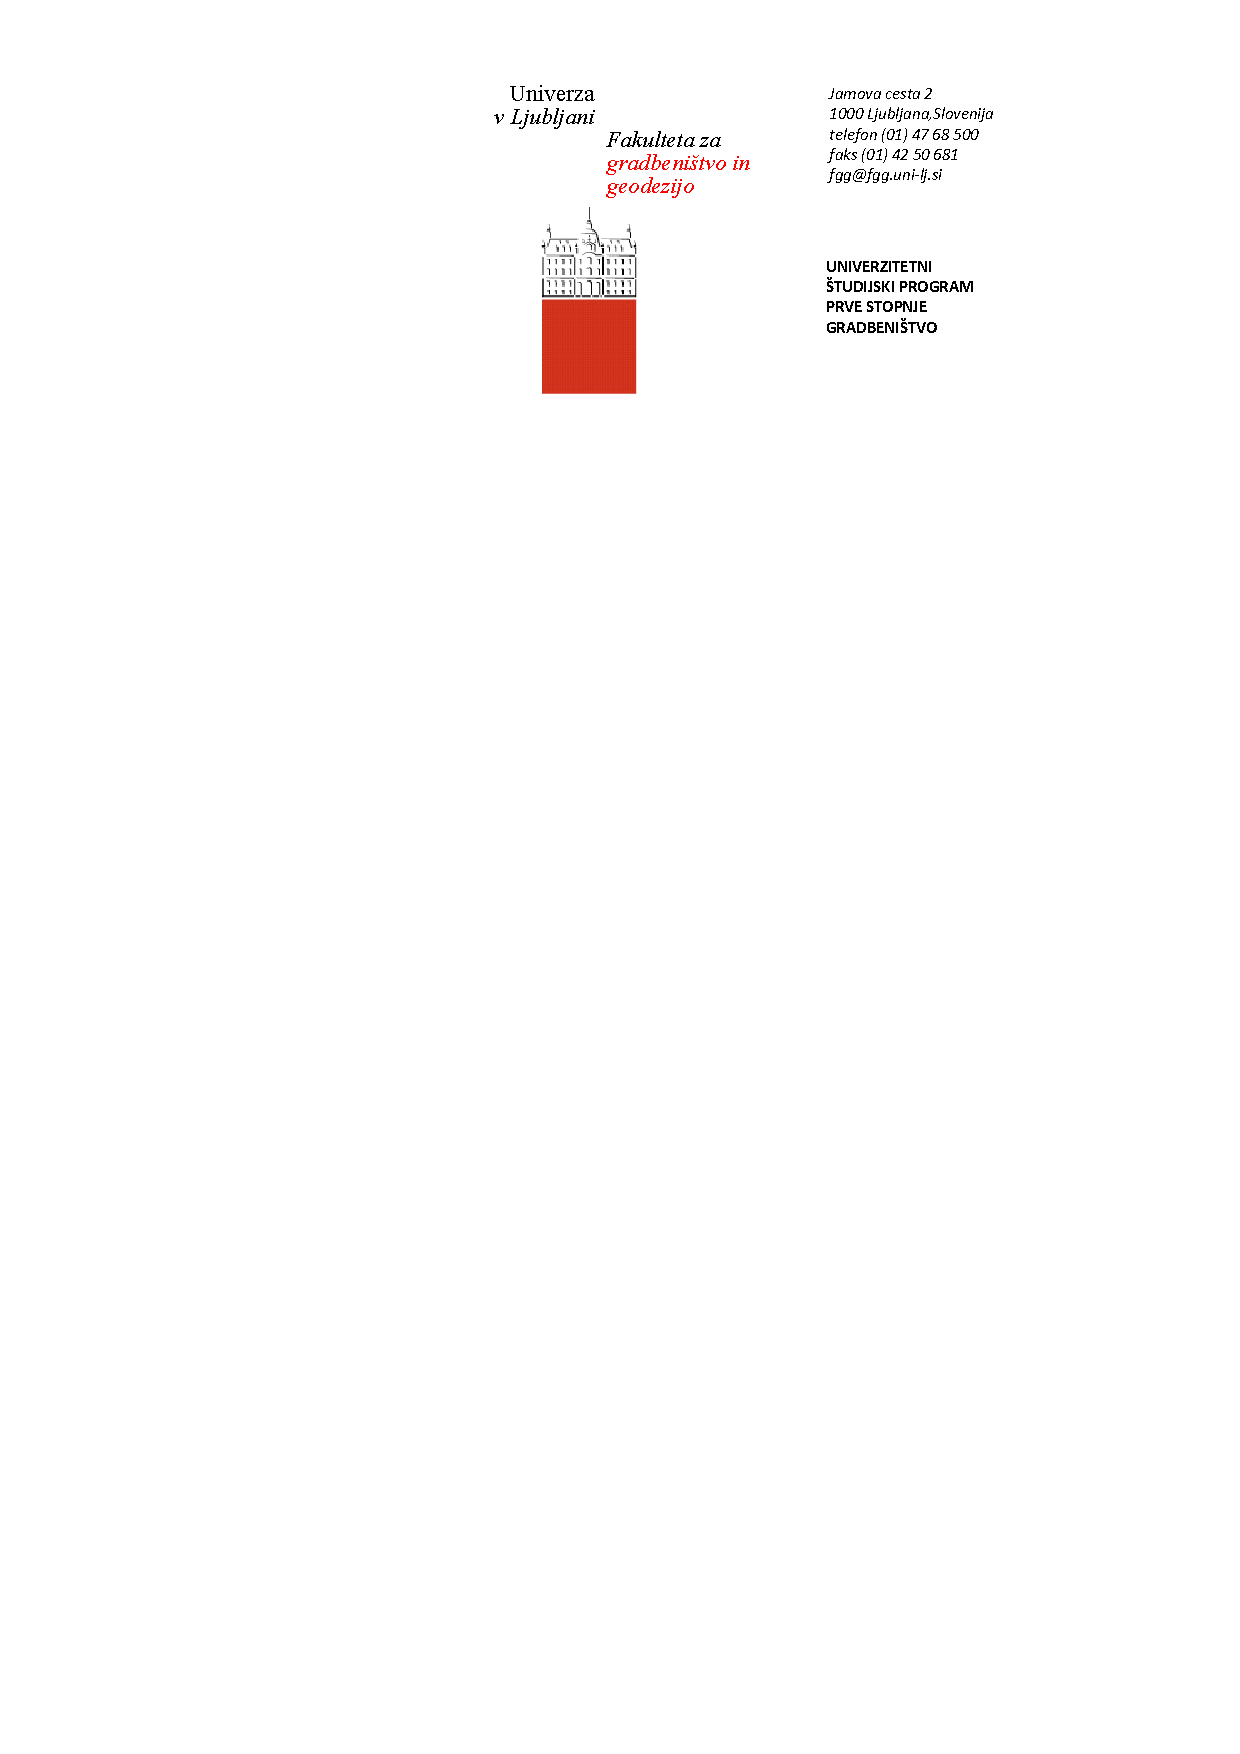
\includegraphics{slike/naslov/logo_faksa_final.pdf}
\end{center}





%\vspace*{5cm}
Kandidat:\\
\vspace*{0.5cm}
\begin{Large}
\textbf{JAN PRIBOŠEK}
\end{Large}

\vspace*{2cm}

\begin{Large}
\textbf{RAČUN ENERGETSKIH PARAMETROV HIDROELEKTRARNE}
\end{Large}

\vspace*{0.5cm}

\begin{large}
\textbf{Diplomska naloga št.:}
\end{large}

\vspace*{1.5cm}

\begin{Large}
	\textbf{CALCULATING ENERGETIC PARAMETERS OF THE HYDROELECTRIC POWER PLANT}
\end{Large}

\vspace*{0.5cm}

\begin{large}
	\textbf{Graduation thesis No.:}
\end{large}



\end{center}
\vspace*{8cm}


% mentor
\begin{large}
	\textbf{Mentor:}\\
	doc. dr. Andrej Kryžanowski \\
\end{large}

\begin{center}
% date
\textsc{Ljubljana, 20.08.2017}
\end{center}

\end{minipage}

\newpage
\thispagestyle{empty}
\cleardoublepage
%
\includepdf[pages={1,{}},offset=1in -1in]{Naslovnica/Platnica.pdf}
%
\includepdf[pages={1},offset=1in -1in]{Naslovnica/PlatnicaZaTisk.pdf}

%------------------------------------
% Prve strani
%------------------------------------
\pagenumbering{Roman}
%
\includepdf[pages={1,{},2,{},3,{}},offset=1in -1in]{Naslovnica/Naslovnica.pdf}
%
\includepdf[pages={1,{},2,{},3,{}},offset=1in -1in]{Naslovnica/NaslovnicaSpodpisom.pdf}

\pagestyle{fancy}
\fancypagestyle{plain}{}
\fancyhf{}
\fancyhead[RO,LE]{\footnotesize \thepage \\}
\fancyhead[LO,RE]{\footnotesize Pribošek, J. 2017. 
Izračun energetskih parametrov hidroelektrarne. \\
Dipl. nal. Ljubljana, UL FGG, 
Univerzitetni študijski program I. stopnje Gradbeništvo.}

\chapter*{POPRAVKI}
\thispagestyle{fancy}

\begin{table}[h!]
\begin{tabularx}{\textwidth}{@{}>{\bfseries}p{4cm} @{}>{\bfseries}p{4cm} @{}>{\bfseries}p{4cm} @{}>{\bfseries}p{4cm}}
%
Stran z napako	& Vrstica z napako	& Namesto & Naj bo	 \\
%
\end{tabularx}
\end{table}
\chapter*{IZJAVE}
\thispagestyle{fancy}

Spodaj podpisani študent \textbf{Jan Pribošek}, vpisna številka \textbf{26110710}, sem avtor pisnega zaključnega dela študija z naslovom: \textbf{Izračun energetskih parametrov hidroelektrarne}

\begin{center}
	IZJAVLJAM
\end{center}

\begin{enumerate}
	\item Obkrožite eno od variant a) ali b)
	
		\begin{enumerate}
			\item da je pisno zaključno delo študija rezultat mojega samostojnega dela
			
			\item da je pisno zaključno delo študija rezultat lastnega dela več kandidatov in izpolnjuje pogoje, ki
			jih Statut UL določa za skupna zaključna dela študija ter je v zahtevanem deležu rezultat
			mojega samostojnega dela
		\end{enumerate}
	
	\item da je tiskana oblika pisnega zaključnega dela študija istovetna elektronski obliki pisnega
	zaključnega dela študija
	
	\item da sem pridobil vsa potrebna dovoljenja za uporabo podatkov in avtorskih del v pisnem
	zaključnem delu študija in jih v pisnem zaključnem delu študija jasno označil
	
	\item da sem pri pripravi pisnega zaključnega dela študija ravnal v skladu z etičnimi načeli in, kjer je to
	potrebno, za raziskavo pridobil soglasje etične komisije
	
	\item soglašam, da se elektronska oblika pisnega zaključnega dela študija uporabi za preverjanje
	podobnosti vsebine z drugimi deli s programsko opremo za preverjanje podobnosti vsebine, ki je
	povezana s študijskim informacijskim sistemom članice
	
	\item da na UL neodplačno, neizključno, prostorsko in časovno neomejeno prenašam pravico shranitve
	avtorskega dela v elektronski obliki, pravico reproduciranja ter pravico dajanja pisnega zaključnega
	dela študija na voljo javnosti na svetovnem spletu preko Repozitorija UL
	
	\item da dovoljujem objavo svojih osebnih podatkov, ki so navedeni v pisnem zaključnem delu študija in
	tej izjavi, skupaj z objavo pisnega zaključnega dela študija.
	
\end{enumerate}

\vfill


V Ljubljani, \today 
\vspace{1cm}

\hspace*{\fill}Jan Pribošek
\chapter*{BIBLIOGRAFSKO-DOKUMENTACIJSKA STRAN IN IZVLEČEK}
\thispagestyle{fancy}
\addcontentsline{toc}{chapter}{BIBLIOGRAFSKO-DOKUMENTACIJSKA STRAN IN IZVLEČEK}

\begin{table}[h!]
\begin{tabularx}{\textwidth}{@{}>{\bfseries}p{3.5cm}@{} @{}>{\bfseries}p{12.5cm}@{}}
%
UDK:	& 620.9:627.8(043.2)					 \\
Avtor: & Jan Pribošek								 \\
Mentor:& doc. dr. Andrej Kryžanowski				 	 \\
Naslov: & Račun parametrov hidroelektrarne \\
Tip dokumenta: & Diplomska naloga - univerzitetni študijski program gradbeništvo 		\\
Obseg in oprema: & {\totalpages} str., {\totalfigures} sl., {\totaltables} pregl., {\totalequations} en. \\
Ključne besede: & Energetski parametri hidroelektrarne, pretok vode, pretok vode v poljubno oblikovani strugi
%

\end{tabularx}
\end{table}

\textbf{Izvleček}

V okviru diplomske naloge sem razvil aplikacijo za računanje energetskih parametrov pretočne hidroelektrarne. V prvem delu naloge sem opisal teoretične osnove za razvoj take aplikacije in opisal princip metod, ki jih aplikacija uporablja za izračun energetskih parametrov pretočne hidroelektrarne. V drugem delu naloge pa sem s primerom dokazal pravilnost algoritma, ki ga aplikacija uporablja.


 \chapter*{BIBLIOGRAPHIC-DOCUMENTALISTIC INFORMATION AND ABSTRACT}
\thispagestyle{fancy}
\addcontentsline{toc}{chapter}{BIBLIOGRAPHIC-DOCUMENTALISTIC INFORMATION AND ABSTRACT}

%
\begin{table}[h!]
\begin{tabularx}{\textwidth}{@{}>{\bfseries}p{3.5cm}@{} @{}>{\bfseries}p{12.5cm}@{}}
%
UDC	& 620.9:627.8(043.2)				 \\
Author: & Jan Pribošek								 \\
Supervisor:& Assist. Prof. Andrej Kryžanowski, Ph. D.			 	 \\
Title: & Calculating energy parameters of the hydroelectric power plant	 \\
Document type: &  Graduation - Thesis - university program \\
Notes: & {\totalpages} p., {\totalfigures} fig., {\totaltables} tab., {\totalequations} eq. \\
Keywords: &  Energy parameters of hydroelectric power plant, river flow, flow in arbitrarily formed river channel
%
\end{tabularx}
\end{table}
\textbf{Abstract}

In thesis I have developed software for calculating parameters of run-of-river hydroelectric power plant. In the first part of the thesis I described the theory basics on which the software is built upon, and described the algorithms for calculating the energy parameters of hydroelectric power plants. In the second part of the thesis, I provided an example that proves correctness of the software calculations and presented the reason why the results differ based on the chosen method of calculations.

%------------------------------------
% Zahvala
%------------------------------------
\chapter*{ZAHVALA}
\thispagestyle{fancy}
\addcontentsline{toc}{chapter}{ZAHVALA}


%------------------------------------
% Kazala
%------------------------------------
%\clearpage
\pdfbookmark{\contentsname}{Contents}
% zaradi rimskih �tevilk raz?irimo ?irino boxa za ?tevilke
% strani v kazalu
\makeatletter
\renewcommand{\@pnumwidth}{2.5em}
\renewcommand{\@tocrmarg}{3em}
\makeatother
\tableofcontents
\thispagestyle{fancy}
%\tocloftpagestyle{fancy}

%\clearpage
\listoffigures
\thispagestyle{fancy}
%\tocloftpagestyle{fancy}


%\clearpage
\listoftables
\thispagestyle{fancy}
%\tocloftpagestyle{fancy}

%\clearpage
%\listofffigure
%\thispagestyle{fancy}
%\tocloftpagestyle{fancy}

%\clearpage
%\listofttable
%\thispagestyle{fancy}
%\tocloftpagestyle{fancy}

%\clearpage
%\listofappendices
%\thispagestyle{fancy}
%\tocloftpagestyle{fancy}

%------------------------------------
% Vsebina
%------------------------------------
\mainmatter
\pagenumbering{arabic}
\pagestyle{fancy}
\fancypagestyle{plain}{}
\fancyhf{}
\fancyhead[RO,LE]{\footnotesize \thepage \\}
\fancyhead[LO,RE]{\footnotesize Pribošek, J. 2017. 
Izračun energetskih parametrov hidroelektrarne. \\
Dipl. nal. Ljubljana, UL FGG, 
Univerzitetni študijski program I. stopnje Gradbeništvo.}



\chapter{Uvod}\label{sec: Uvod}
\thispagestyle{fancy}


Letna količina vode ki se pretoči v Sloveniji je 33,9 $km^{3}$, kar nas primerjano na število prebivalcev uvršča v sam vrh v Evropi, takoj za Švico in Norveško. Potreba po električni energiji se iz leta v leto veča, vendar se le okoli 47\% vodnega potenciala efektivno uporablja za potrebe proizvodnje električne energije. Voda v Sloveniji je povsod okoli nas, zato je zanimivo preračunati koliko električne energije bi lahko proizvedli iz bližnjega potoka ali večje reke. Podatki o pretokih rek v Sloveniji so namreč javno dostopni v arhivu na spletni strani agencije Republike Slovenije za okolje (ARSO). \cite{HEnaSrednjiSavi}


Cilj diplomske naloge je izdelava aplikacije, ki omogoča oceno hidroenergetskega potenciala vodotoka na poljubnem odseku. Vhodni podatek predstavljajo povprečni dnevni pretoki, ki so na voljo iz javno dostopnih podatkovnih baz in parametri rečne struge, ki jih določimo iz razpoložljivih geodetskih podatkov (karakteristični prečni prerezi in naklon struge) in podatkov iz literature (koeficient hrapavosti). Aplikacija omogoča, da s pomočjo začetno ocenjenih parametrov struge in razpoložljivih povprečnih dnevnih pretokov na izbranem odseku vodotoka izračunamo energetske parametre pretočne hidroelektrarne.


V diplomski nalogi bomo najprej opisali postopek izračuna z osnovnimi enačbami, na koncu pa bomo primerjali rezultate ročnega izračuna z rezultati ki jih izračuna program. Pri izračunu smo upoštevali, da je gladina vode v zadrževalniku za pregrado na maksimalni konstantni višini, izkoristek elektrarne konstanten in neodvisen od obratovalnega pretoka ter naklon struge od 0\% do 2\%.



%-----------------------------------------------------------

\chapter{Teoretične osnove}

Parametre za iskano hidroelektrarno lahko izračunamo po naslednjem algoritmu:
\begin{enumerate}[noitemsep, topsep=0pt]
	\item Pridobitev podatkov
	\item Analiza hidrološkega niza podatkov za iskano obdobje
	\item Izračun konsumpcijske krivulje
	\item Izračun proizvodnje električne energije
\end{enumerate}


%-------------------------------------
\section{Pridobitev podatkov}
Za nadaljnje izračune potrebujemo podatke o:
\begin{itemize}[noitemsep, topsep=0pt]
	\item Dimenzijah in naklonu rečne struge
	\item Manningovem koeficientu hrapavosti rečnega korita
	\item Povprečnih dnevnih pretokih vodotoka za izbrano obdobje
\end{itemize}

Podatke o dimenzijah rečnega korita lahko pridobimo z meritvami na terenu ali pa dimenzije ocenimo na podlagi ortofoto posnetkov. Naklon rečne struge vodotoka se lahko oceni s pomočjo spletne aplikacije Geopedija. Izberemo odsek vodotoka, ki ga definirata dve točki. S pomočjo Geopedije odčitamo podatke o višinski razliki $\Delta h$ in razdalji $\Delta L$ med točkama. S pomočjo spodnje enačbe določimo naklon izbranega odseka vodotoka:

\begin{ceqn}
\begin{align}
 I = \dfrac{100\Delta h}{\Delta L} [\%]
\end{align}
\end{ceqn}


  Manningov koeficient hrapavosti rečnega korita $ng$ se lahko oceni izkustveno na terenu s pomočjo priročnikov ali pa z umerjanjem na podlagi podatkov o nivojih vode in pretokih. Manningov koeficient hrapavosti je odvisen od naslednjih 7 faktorjev \cite{VenTeChow}:
 \begin{enumerate}[noitemsep, topsep=0pt]
 	\item Hrapavosti površine ostenja
 	\item Zaraščenosti rečnega korita
 	\item Neregularnosti oblike rečnega korita
 	\item Meandriranja rečne struge
 	\item Zamašitve struge s plavinami 
 	\item Oblike in velikosti rečnega korita
 	\item Polnosti rečnega korita z vodo
 \end{enumerate}
 

 
 
  Podatke o pretokih slovenskih vodotokov lahko pridobimo iz arhiva, ki se nahaja na spletni strani agencije Republike Slovenije za okolje (v nadaljevanju ARSO). V primeru da iščemo pretok za manjši vodotok, je zelo verjetno da podatki o pretokih vodotoka ne obstajajo. V tem primeru lahko pretok vodotoka ocenimo s pomočjo meritev višine gladine vode in dimenzij struge, ocene Manningovega koeficienta hrapavosti in naklona struge. S pomočjo Manningove enačbe opisane kasneje v poglavju~\ref{sec:teorija_trapeznaMetoda} in prej omenjenih členov Manningove enačbe dobimo končno ocenjeno vrednost pretoka vodotoka za posamezno obdobje meritev.




%------------------------------------------------
\section{Analiza hidrološkega niza podatkov}
%TODO: FIXME -> izboljšaj
Iz ARSO-vega arhiva lahko izvozimo podatke o povprečnih dnevnih pretokih iskanega vodotoka v csv obliki (comma separated values). Iz izvoženih podatkov lahko za vsak mesec obdobja izračunamo povprečni mesečni pretok. Če mesečne pretoke povprečimo za vsa leta izbranega obdobja lahko navedene povprečne mesečne pretoke obdobja prikažemo na hidrogramu obdobja. Hidrogram je graf, ki prikazuje povprečne mesečne pretoke vodotoka za izbrano obdobje analize.  %Prav tako se lahko določi mokro in suho leto obdobja, ki ju primerjamo s povprečnimi mesečnimi pretoki.

%TODO: krivulja trajanja



%------------------------------------------------
\section{Izračun konsumpcijske krivulje}
Konsumpcijska krivulja je graf funkcije, ki predstavlja višino gladine vode v odvisnosti od pretoka vode v rečni strugi. Graf konsumpcijske krivulje potrebujemo za določitev višinske razlike $dh$ med spodnjo in zgornjo vodo hidroelektrarne v odvisnosti od pretoka vode skozi turbine hidroelektrarne. Višinsko razliko $dh$ potrebujemo za določitev moči hidroelektrarne v zadnjem koraku algoritma opisanega v tem poglavju.



%-------------------------------------------------
\subsection{Izračun konsumpcijske krivulje za pravokotne in trapezne struge} \label{sec:teorija_trapeznaMetoda}
Za izračun konsumpcijske krivulje potrebujemo pretok vodotoka $Q$ v odvisnosti od višine gladine vode $h$ v strugi. Gladina vode $h$ poteka od dna struge do maksimalne višine struge vodotoka $H$. Pretok vode v strugi $Q$ se za vsak cm višine $h$ izračuna po Manningovi enačbi:

\begin{ceqn}
\begin{align}
Q(h) = \dfrac{1}{ng} \sqrt{I}\dfrac{S(h)^{5/3}}{P(h)^{2/3}} \label{eq:ManningovaEnacba}
\end{align}
\end{ceqn}

Kjer je:

\begin{table}[htb!]
	\begin{tabular}{r|p{10cm}}
		Q & pretok \\
		ng & Manningov koeficient hrapavosti dna struge\\
		I & naklon struge \\
		S & ploščina omočenega dela prečnega profila \\
		P & dolžina omočenega oboda struge
	\end{tabular}
\end{table}


\newpage
% pravokotna struga
\begin{enumerate}
	\item Pravokotno oblikovana struga vodotoka:
	
	\begin{figure}[H]
		\begin{centering}
			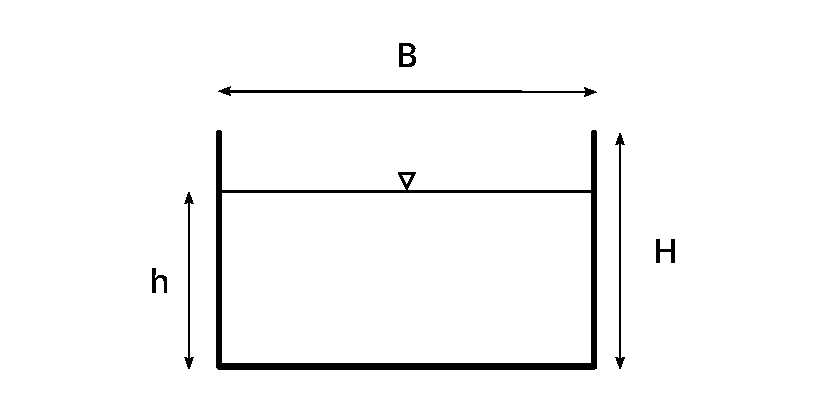
\includegraphics{slike/konsumpcijska_krivulja/rectangularChannel.pdf}		
			\caption{Prečni prerez pravokotne struge}\label{fig:pravokotna struga}
		\end{centering}
	\end{figure}
	

	Omočeni obod pravokotne struge izračunamo kot seštevek širine dna struge in dvakratne višine gladine vode v strugi vodotoka $h$.
	
	\begin{ceqn}
	\begin{equation}
	P_{p}(h) = B + 2h
	\end{equation}
	\end{ceqn}
	
	Ploščino omočenega dela, ki ga omejujejo rečno korito in gladina vode za pravokotno oblikovano rečno strugo dobimo po enačbi:
	
	\begin{ceqn}
	\begin{align}
	S_{p}(h) = B \cdot h
	\end{align}
	\end{ceqn}
	
	\item Trapezno oblikovana struga vodotoka:
	
		\begin{figure}[ht!]
			\begin{centering}
				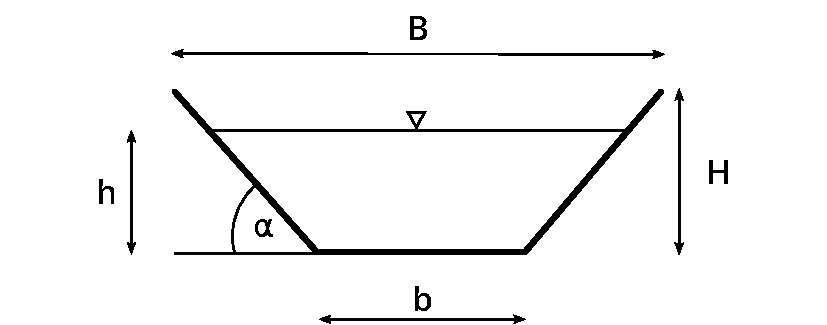
\includegraphics{slike/konsumpcijska_krivulja/trapezoidChannel.pdf}		
				\caption{Prečni prerez trapezne struge}\label{fig:trapezna struga}
			\end{centering}
		\end{figure}
	
	Omočeni obod trapezno oblikovane rečne struge izračunamo kot seštevek širine dna struge in dvakratne razdalje od roba dna do točke presečišča rečnega korita z gladino vode:
	
	\begin{ceqn}
	\begin{align}
	P_{t}(h) = b + 2 \cdot \sqrt{h^2 + \left(\dfrac{h} {\tan\alpha} \right)^{2}}
	\end{align}
	\end{ceqn}
	
	Ploščino omočenega dela v trapezno oblikovani rečni strugi izračunamo po enačbi:
	\begin{ceqn}
	\begin{align}
	S_{t}(h) = b \cdot h + \dfrac{h^2}{ 2\tan\alpha}
	\end{align}
	\end{ceqn}
	
\end{enumerate}



Ko poznamo vse parametre Manningove enačbe \ref{eq:ManningovaEnacba}, izračunamo pretoke vodotoka za vsak cm višine rečne struge, ki poteka od višine 0 do $H$ in narišemo graf konsumpcijske krivulje $h(Q)$.


\newpage
%------------------------------------------------
\subsection{Izračun konsumpcijske krivulje za struge poljubne oblike}\label{sec:pretokNumericnaMetoda}


V primeru da iščemo konsumpcijsko krivuljo za vodotok poljubne oblike, si za izračun le te ne moremo pomagati s znanimi formulami preprostih geometrijskih likov. Poljubno oblikovano strugo lahko popišemo s serijo točk, ki jih dodajamo v kartezijski koordinatni sistem. Za vsako točko ki definira poljubno rečno korito podamo x in y koordinato, za točke pa predpostavimo da so med seboj povezane z enačbo linearne funkcije. Na sliki~\ref{fig:poljubnaStruga} je predstavljen prečni prerez poljubno oblikovane struge vodotoka.

\begin{figure}[ht!]
	\begin{centering}
		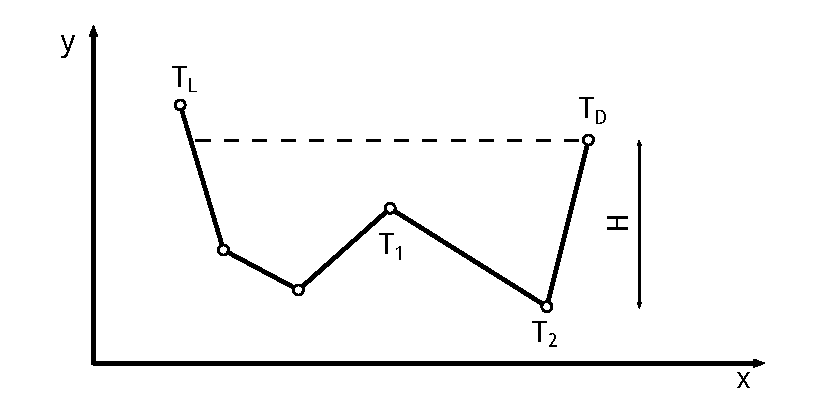
\includegraphics{slike/customChannel/customStruga.pdf}		
		\caption{Prečni prerez poljubno oblikovane struge vodotoka}\label{fig:poljubnaStruga}
	\end{centering}
\end{figure}



%------------------------------------------
%\subsection{Izračun višine rečnega korita}
Skrajni točki na robu struge sta točki $T_L$ in $T_D$ na sliki \ref{fig:poljubnaStruga}. Točko na robu struge z nižjo y koordinato označimo s $T_{Rmin}$ (na sliki \ref{fig:poljubnaStruga} označena kot točka $T_D$). Najnižjo točko struge vodotoka označimo s $T_{min}$. Maksimalna gladina vode v rečnem koritu $H$ je definirana kot razdalja med točkama $T_{Rmin}$ in $T_{min}$. V primeru da je višina gladine vode večja od višine rečnega korita $H$ pride do preliva vode čez robove rečnega korita.



%\subsection{Določitev parametrov odseka}
Za določitev parametrov odseka, ki jih potrebujemo za izračun konsumpcijske krivulje, s točkami definirano poljubno strugo vodotoka najprej razdelimo na odseke po dve točki $O_1$ ($x_1$, $y_1$) in $O_2$ ($x_2$, $y_2$). Za vsak izbran odsek rečne struge, se najprej določi enačba linearne funkcije, ki povezuje točki $O_1$ in $O_2$.

Enačba linearne funkcije se definira kot:
\begin{ceqn}
\begin{align}
f(x) = kx + n \label{eq:enacba_linearnafunkcija}
\end{align}
\end{ceqn}

Naklon funkcije k se izračuna po spodnji enačbi:

\begin{ceqn}
\begin{align}
k = \dfrac{y_2 - y_1}{x_2 - x_1}
\end{align}
\end{ceqn}



Če v enačbo linearne funkcije \ref{eq:enacba_linearnafunkcija} vstavimo izračunan naklon $k$ in koordinate točke $O_1$, lahko izračunamo iskani $n$. S tem je določena enačba linearne funkcije $f(x)$ ki povezuje točki $O_1$ in $O_2$.

\begin{figure}[H]
	\begin{centering}
		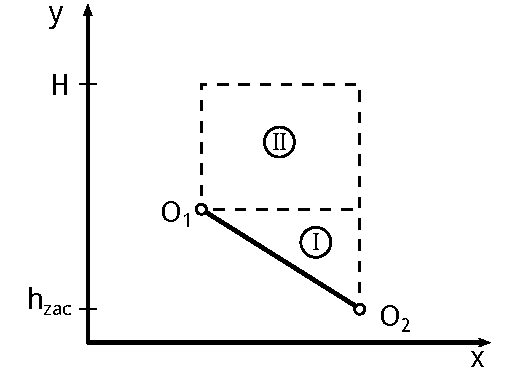
\includegraphics{slike/customChannel/odsek.pdf}
		\caption{Izbrani odsek struge} \label{fig:odsekStruge}
	\end{centering}
\end{figure}








% določitev ploščine posameznega kosa
Za vsak odsek dveh točk se določi najnižja točka odseka $T_z$, na sliki \ref{fig:odsekStruge} označena kot točka $O_2$. Y koordinata točke $T_z$ nam predstavlja začetno višino odseka $h_{z}$. Od $h_z$ do končne višine gladine rečnega korita H za vsak cm po višini določimo presečišče $G$ prej izračunane funkcije $f(x)$ s horizontalno ravnino $g = h$, ki predstavlja gladino vode pri trenutni višini $h$, kar je prikazano na sliki \ref{fig:custom_odsekDetajl}.


%FIXME-URGENT -> Računanje S in P glede na pozicijo presečišča G


\begin{figure}[ht!]
	\begin{centering}
		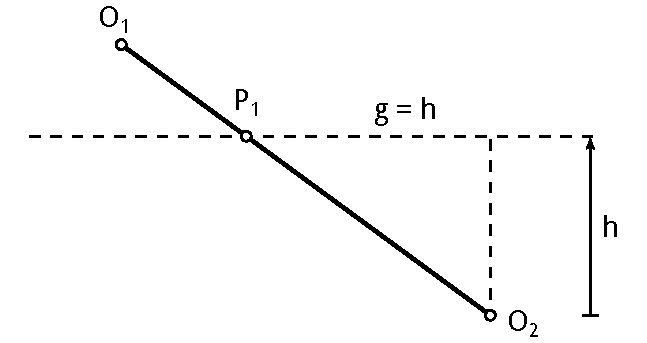
\includegraphics{slike/customChannel/odsek_detajl.pdf}
		\caption{Detajl odseka struge}\label{fig:custom_odsekDetajl}
	\end{centering}
\end{figure}



Ko imamo določeno presečišče $G$ gladine vode s funkcijo $f(x)$ med točkama odseka, lahko izračunamo dolžino omočenega oboda struge odseka in ploščino lika ki ga oklepajo funkcija odseka $f(x)$, navidezna gladina vode $g = h$ in najnižja točka odseka $T_z$, na sliki \ref{fig:odsekStruge} označena z $O_2$. Zaradi poenostavljenega zapisa so v nadaljevanju koordinate točke $O_1$ označene kot $x_1$ in $y_1$, koordinate točke $O_2$ pa $x_2$ in $y_2$.


Način izračuna omočenega oboda struge vodotoka $P(h)$ in ploščine prečnega prereza $S(h)$ je odvisen od pozicije presečišča $G$:


\begin{enumerate}
	\item V primeru da se presečišče $G$ izbranega odseka struge nahaja v območju med točkama $O_1$ in $O_2$, dolžino omočenega oboda določimo po Pitagorovem izreku kot:
		
	%FIXME: decide on index G_x or Gx
	\begin{ceqn}
		\begin{align}
		P(h) = \sqrt{(T_{zx} - G_x(h))^{2} + (T_{zy} - G_y(h))^{2}}
		\end{align}
	\end{ceqn}
	
	
	Ploščino območja ki ga oklepajo horizontalna ravnina s presečiščem $G$ in najnižjo točko odseka $T_z$ pa določimo kot ploščino trikotnika (območje I na sliki~\ref{fig:odsekStruge}) po formuli:
	
	\begin{ceqn}
	\begin{align}
	S(h) = \dfrac{|T_{zx} - G_x(h)| \cdot |T_{zy} - G_y(h)|}{2}
	\end{align}
	\end{ceqn}
	
	
	\item V primeru, da se presečišče $G$ nahaja izven območja točk $O_1$ in $O_2$ se dolžina omočenega oboda odseka izračuna kot razdalja med točkama $O_1$ in $O_2$ po Pitagorovem izreku:
	
	\begin{ceqn}
	\begin{align}
	P = \sqrt{ (x_1 - x_2)^{2} + (y_1 - y_2)^{2}}
	\end{align}
	\end{ceqn}
	
	Ploščina $S$ odseka pa se določi kot seštevek ploščin območij I in II na sliki \ref{fig:odsekStruge}.
	
	\begin{ceqn}
	\begin{align}
	S(h) = S_I + S_{II}(h)
	\end{align}
	\end{ceqn}
	
	Pri čemer je $S_I$ enak:
	
	\begin{enumerate}
		
		
		\item V primeru če je naklon funkcije $f(x)$, $k = 0$ se ploščina $S_I$ izračuna kot:
		\begin{ceqn}
			\begin{align}
			S_I(h) = \bigg|(x_2 - x_1) \cdot (h - y_1)\bigg|
			\end{align}
		\end{ceqn}
		
		
		\item Če za naklon funkcije $f(x)$ velja $k \neq 0$:
		
			\begin{ceqn}
				\begin{align}
				S_I(h) = \bigg|\dfrac{ (y_2 - y_1) \cdot  (x_2 - x_1)}{2}\bigg|
				\end{align}
			\end{ceqn}
			

	\end{enumerate}

	
	
	 $S_{II}$ pa se izračuna kot:
	
	\begin{ceqn}
	\begin{align}
	\\
	S_{II}(h)&= \bigg|(x_2 - x_1) \cdot (h - y_1)\bigg|
	\end{align}
	\end{ceqn}

	
\end{enumerate}


Ko imamo za vsak cm višine gladine vode izračunan omočeni obod $P_n(h)$ odseka $n$ in ploščino prečnega prereza pod gladino vode $S_n(h)$ lahko določimo pretok vode skozi odsek $Q_n(h)$. Pretok vode skozi odsek izračunamo po Manningovi enačbi \ref{eq:ManningovaEnacba}. Za vsak računani odsek moramo poznati tudi naklon struge vodotoka $I_n$ in  Manningov koeficient hrapavosti površine $ng_n$.


\begin{ceqn}
	\begin{align}
	Q_n(h) = \dfrac{1}{ng_n} \sqrt{I_n}\dfrac{S_n(h)^{5/3}}{P_n(h)^{2/3}}
	\end{align}
\end{ceqn}


Ko imamo posamezne pretoke po višinah za vse odseke izračunane, jih medsebojno seštejemo in dobimo končne vrednosti pretokov $Q(h)$:

\begin{ceqn}
\begin{align}
Q(h) = Q_1(h) + Q_2(h) + Q_3(h) + ... + Q_{n-1}(h) + Q_n(h)
\end{align}
\end{ceqn}


S imamo točke za izris konsumpcijske krivulje določene in funkcijo konsumpcijske narišemo na graf $h(Q)$.



\newpage

\section{Izračun proizvodnje električne energije}
Za določitev končne proizvodnje električne energije potrebujemo razliko med koto zgornje vode t.j. vode v rezervoarju in koto spodnje vode, ki jo določimo iz grafa konsumpcijske krivulje izračunanega za izbrano strugo.

\begin{figure}[ht!]
	\begin{centering}
		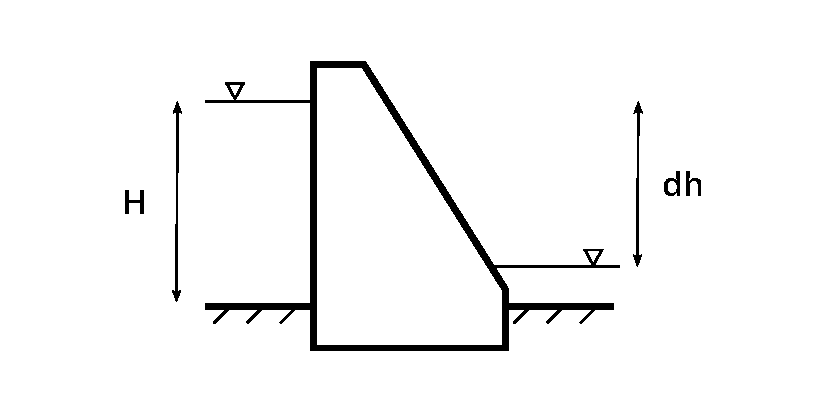
\includegraphics{slike/electricityProduction/powerplant_crossSection.pdf}
		\caption{Shema prečnega prereza hidroelektrarne}
	\end{centering}
\end{figure}

Ker računamo proizvodnjo električne energije za pretočne hidroelektrarne, predpostavimo da je kota zgornje vode konstantna na višini $H$. Koto spodnje vode določimo iz prej izračunane konsumpcijske krivulje iz katere odčitamo višino spodnje vode v strugi za dani povprečni mesečni pretok skozi turbino hidroelektrarne. V primeru da se pretok skozi turbino hidroelektrarne nahaja med dvema točkama pretokov v konsumpcijski krivulji, iskano višino spodnje vode določimo z linearno interpolacijo med znanima točkama na grafu konsumpcijske krivulje.

Višinsko razliko med koto zgornje in spodnje vode določimo po spodnji enačbi:

\begin{ceqn}
\begin{align}
dh = H - H_{spodaj}
\end{align}
\end{ceqn}

Moč hidroelektrarne izračunamo po enačbi:

\begin{ceqn}
\begin{align}
P = \mu \cdot g \cdot Q \cdot dh
\end{align}
\end{ceqn}

Pri čemer so:
\begin{table}[htb!]
	\begin{tabular}{r|p{10cm}}
		P & moč [$kW$]\\
		$\mu$ & izkoristek turbine [\%]\\
		g & gravitacijska konstanta [$9,81\dfrac{m}{s^{2}}$ ] \\
		Q & pretok [$m^{3}/s$]\\
		dh & razlika višin spodnje in zgornje vode [$m$]
	\end{tabular}
\end{table}


Za določitev končne mesečne proizvodnje električne energije, za vsak mesec določimo povprečno moč $\overline{P}$ in uporabimo naslednjo enačbo

\begin{ceqn}
\begin{align}
E = \dfrac{24 \cdot \overline{P} \cdot d}{1000}
\end{align}
\end{ceqn}

Pri čemer so:
\begin{table}[htb!]
\begin{tabular}{r|p{10cm}}
	E & proizvedena električna energija [$MWh$]\\
	$\overline{P}$ & povprečna moč v mesecu [$kW$]\\
	d & število dni v mesecu \\
\end{tabular}
\end{table}



\chapter{Izračun}


V tem poglavju bom s primerom dokazal, da program računa parametre pretočne hidroelektrarne pravilno. Za dokaz bom uporabil namišljen primer trapezno oblikovane struge vodotoka prikazane na sliki \ref{fig:izracun_trapeznaStruga} z Manningovim koeficientom hrapavosti 0,3 in z 1\% naklonom struge. Rezultate ročnega izračuna primerjal z rezultati ki jih izračuna program po trapezni metodi in numerični metodi opisani v poglavju \ref{sec:pretok_prav_trapez}  oz. \ref{sec:pretokNumericnaMetoda}.



\begin{figure}[ht!]
	\begin{centering}
		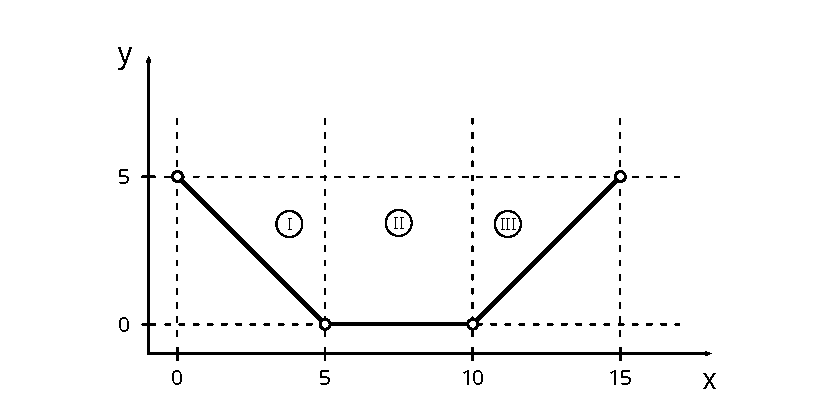
\includegraphics[width=\textwidth]{slike/izracuni/trapeznaStruga.pdf}		
		\caption{Struga vodotoka katerega bomo preračunali}\label{fig:izracun_trapeznaStruga}
	\end{centering}
\end{figure}

\section{Ročni izračun parametrov hidroelektrarne}

\begin{enumerate}[I.]
	
	\item Odsek
	
		\begin{align}
			S_I = \dfrac{5 * 5}{2} = 12,5
		\end{align}
		
		\begin{align}
			P_I = \sqrt{5^2 + 5^2} = 7,07
		\end{align}
		
		\begin{align}
			Q_1 = \dfrac{\sqrt{0,01}}{0,03} * \dfrac{12,5^{5/3}}{7,07^{2/3}} = 
		\end{align}
	
	
\end{enumerate}


aa


\section{Izračun parametrov hidroelektrarne s programom}

S pomočjo uporabniškega vmesnika v koordinatni sistem vnašamo serijo točk, ki predstavljajo robove izbrane struge. V tabeli na levi strani diagrama, za vsak odsek med dvema točkama dodajamo Manningove koeficiente hrapavosti $ng$ in naklone struge na sliki označene s $\varphi$. V našem primeru so vrednosti koeficientov za vse odseke rečne struge enake.

\begin{figure}[ht!]
	\begin{centering}
		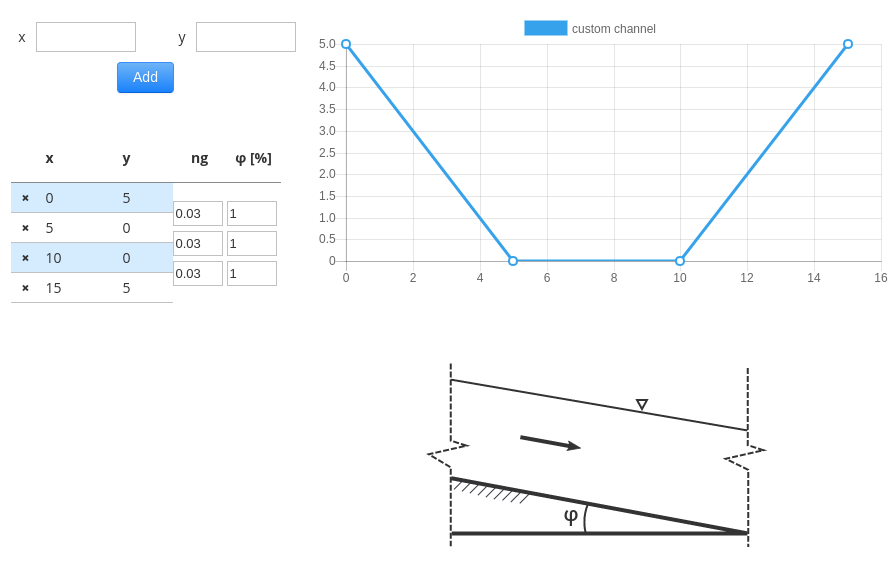
\includegraphics[width=\textwidth]{slike/izracuni/modeliranjeStruge.png}		
		\caption{Vnos podatkov v program}\label{fig:modeliranjeStruge}
	\end{centering}
\end{figure}



\iffalse
%%%%%%%%%%%%%%%%%%%%%%%%%%%%%%%%%%%%%%%%%%%%%%%%%%%%%%%%%%%%
\chapter{FORMULACIJA PROSTORSKIH NOSILCEV PO GEOMETRIJSKO TO?NI 
		 TEORIJI Z NEZVEZNO KINEMATIKO}
%%%%%%%%%%%%%%%%%%%%%%%%%%%%%%%%%%%%%%%%%%%%%%%%%%%%%%%%%%%%
\thispagestyle{fancy}



%-----------------------------------------------------------
\section{Matemati?ni model nosilca}
\label{sec: Matematicni model}
%-----------------------------------------------------------

%
%\begin{figure}[ht]
%\begin{center}
%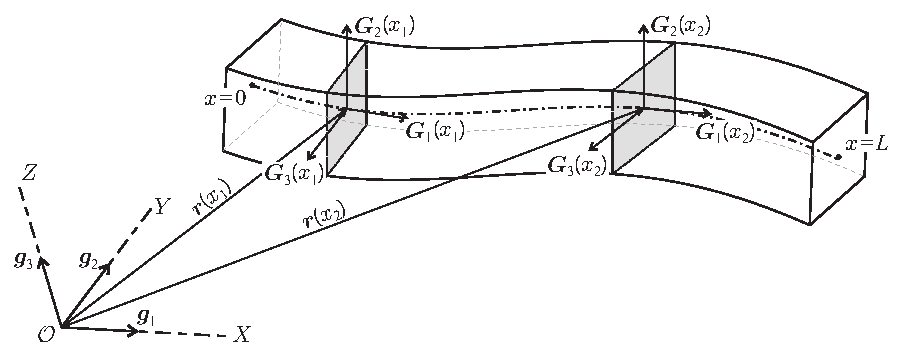
\includegraphics{FormulacijaZNezveznoKinematiko/slike/ModelNosilca}
%\bicaption[fig: Matematicni model nosilca]{}{
%Matemati�ni model nosilca.
%}{Figure}{
%Mathematical beam model.}
%\addfiguretolof{Mathematical beam model.}
%\end{center}
%\end{figure}
%




Vpeljemo dve bazi:
\begin{itemize}
\vspace*{-0.3cm}
\item[(i)] 	Prva je glede na prostor nepomi?na ortonormirana baza $\bs{g}$, 
			ki jo dolo?a trojica 
		    baznih vektorjev $\left\lbrace \bs{g}_1,\bs{g}_2,\bs{g}_3 \right\rbrace$,
		    pripetih v opazovali??e prostora. Nepomi?no bazo v literaturi imenujejo 
		    tudi prostorska ali globalna baza. Matrike, zapisane glede na prostorsko 
		    bazo, ozna?ujemo z indeksom $g$.
\vspace*{-0.7cm}		   
\item[(ii)] Druga je telesna baza 
			$\bs{G} = \left\lbrace \bs{G}_1(x),\bs{G}_2(x),\bs{G}_3(x) \right\rbrace$, 
			ortonormalna. V literaturi jo imenujejo tudi pomi?na ali lokalna baza. 
			Matrike, zapisane glede na telesno bazo, ozna?imo z indeksom $G$.
			Ker je njena pozicija v prostoru odvisna od trenutne rotacije pre?nega 
			prereza, je v splo?nem za vsak pre?ni prerez druga?na, torej odvisna od $x$. 
			Vektorji telesne baze so izbrani tako, da je vektor $\bs{G}_1$ pravokoten na 
			zavrteni pre?ni prerez, bazna vektorja $\bs{G}_2$ in $\bs{G}_3$ pa sta 
			usmerjena vzdol? glavnih vztrajnostnih osi prereza.
\end{itemize} 


\vspace*{-0.3cm}


%-----------------------------------------------------------
\section{Pomiki, rotacije in deformacije}
\label{sec: Pomiki, rotacije in deformacije}
%-----------------------------------------------------------
Geometrijsko to?na teorija reducira tenzorsko polje deformacij, ki je zvezno
porazdeljeno po volumnu nosilca, na dve deformacijski vektorski polji, vezani na 
materialne to?ke osi nosilca \cite{Reissner1981} - vektor translacijskih 
(vzdol?nih, pre?nih) deformacij in vektor rotacijskih deformacij  
(upogib, torzija), ki ju v matri?ni obliki ozna?imo z $\bs{\gamma}_G$ in $\bs{\kappa}_G$.
Njune komponente, $\gamma_1, \gamma_2, \gamma_3$  in 
$\kappa_1, \kappa_2, \kappa_3$, predstavljajo v trenutni telesni 
bazi pre?nega prereza $G$ osno in stri?ni deformaciji, 
torzijski zasuk in upogibni deformaciji - pseudoukrivljenosti. 
Iz principa virtualnega dela sledi, da krajevni vektor vzdol?ne osi nosilca  
in rotacijski vektor pre?nega prereza, ki ju v matri?ni obliki ozna?imo z $\bs{r}_{g}$ 
in $\bs{\vartheta}_{g}$, kakor tudi njuni variaciji 
$\delta\bs{r}_{g}$ in $\delta \bs{\vartheta}_{g}$, zado??ajo pogoju:
%
\begin{align}
\delta\bs{r}'_{g}\left( x \right) &= 
\bm{R}\left(x\right)\delta \bs{\gamma}_{G}\left( x \right) - 
\bs{r}'_{g}\left( x\right) \times
\delta \bs{\vartheta}_{g}\left( x \right) ,
\label{eq: sibka kinematicna enacba 1} \\
\delta\bs{\vartheta}'_{g}\left(x\right) &=
\bm{R}\left(x\right)
\delta\bs{\kappa}_{G} \left(x\right).
\label{eq: sibka kinematicna enacba 2}
\end{align}
%

Z integracijo ena?b \eqref{eq: sibka kinematicna enacba 1} in
\eqref{eq: sibka kinematicna enacba 2} glede na variacije dobimo zveze med krajevnim vektorjem in vektorji 
pomikov, rotacij in deformacij:
%
\begin{align}
\bs{r}'_{g}\left(x\right) & = \bm{R}\left(x\right)
\left( \bs{\gamma}_{G}\left(x\right) - \bs{\gamma}_{G}^{0} \left(x\right)\right),
\label{eq: kinematicna enacba 1} \\
\bs{\vartheta}'_{g}\left(x\right) &= \bm{T}^{-T} \left(x\right)
\left( \bs{\kappa}_{G}\left(x\right)-  \bs{\kappa}_{G}^{0} \left(x\right)\right).
\label{eq: kinematicna enacba 2}
\end{align}
%

\fi

%\include{AproksimacijaPoMKE/AproksimacijaPoMKE}
%\include{NumericniPrimeri/NumericniPrimeri}


%%%%%%%%%%%%%%%%%%%%%%%%%%%%%%%%%%%%%%%%%%%%%%%%%%%%%%%%%%%%
\chapter{ZAKLJUČEK}
%%%%%%%%%%%%%%%%%%%%%%%%%%%%%%%%%%%%%%%%%%%%%%%%%%%%%%%%%%%%
%\thispagestyle{fancy}


Predstavljena formulacija končnih elementov ...

\chapter*{POVZETEK}
\addcontentsline{toc}{chapter}{POVZETEK}

V disertaciji obravnavamo problem...


%\chapter*{SUMMARY}
\addcontentsline{toc}{chapter}{SUMMARY}

In the present dissertation we study ...



%------------------------------------
% Bibliografija
%------------------------------------
\phantomsection
\addcontentsline{toc}{chapter}{VIRI}
\bibliographystyle{disertation}
\bibliography{Bibliografija/Viri}
\thispagestyle{fancy}


%------------------------------------
% Priloge
%------------------------------------
\newpage
\phantomsection
%\chapter*{PRILOGE}
\addcontentsline{toc}{chapter}{DODATKI}
%\listofappendices
\thispagestyle{fancy}
%\appendix
\newcounter{Priloge}
\pagestyle{fancy}
\fancyhf{}
\fancyhead[RO,LE]{\footnotesize \Alph{Priloge}\thepage \\}
\fancyhead[LO,RE]{\footnotesize Pribošek, J. 2017.  \\
Dipl. nal. Ljubljana, UL FGG, 
Univerzitetni študijski program I. stopnje Gradbeništvo.}
\renewcommand{\thechapter}{\Alph{Priloge}}
\renewcommand{\theequation}{\Alph{Priloge}.\arabic{equation}}
%\stepcounter{Priloge}
\setcounter{equation}{0}
\setcounter{page}{1}
%%%%%%%%%%%%%%%%%%%%%%%%%%%%%%%%%%%%%%%%%%%%%%%%%%%%%%%%%%%%
\chapter{PROSTORSKE ROTACIJE}
\label{ch: Dodatek A}
\addcontentsline{loapp}{appendices}{A: PROSTORSKE ROTACIJE}
%%%%%%%%%%%%%%%%%%%%%%%%%%%%%%%%%%%%%%%%%%%%%%%%%%%%%%%%%%%%
\thispagestyle{fancy}

%Na tem mestu povzamemo dejstva o rotacijah in operacijah, povezanih z njimi, 
%ter izpeljave, ki jih potrebujemo v okviru tega dela. Ob�iren pregled podro�ja 
%rotacij je v svoji doktorski disertaciji predstavil Zupan \cite{ZupanPhd2003}. 
%Ker so rotacije pomemben del prostorskih problemov v mehaniki, jih obravnavajo 
%tudi v mnogih u�benikih in publikacijah (npr. Crisfield \cite{CrisfieldFE1997}, 
%Argyris \cite{Argyris1982}, Alturi in Cazzani \cite{AlturiCazzani1995}).


%-----------------------------------------------------------
\section{Rotacijska matrika}
\label{sec: Rotacijska matrika}
%-----------------------------------------------------------
V razdelku \ref{sec: Matematicni model} smo vpeljali prostorsko in telesno bazo 
prostora. Preslikava med obema ortonormiranima bazama, ki ju uporabljamo 
za opis prostorskega nosilca, je rotacija 
$R: \left\lbrace \bs{g}_{1}, \bs{g}_{2}, \bs{g}_{3} \right\rbrace
\longrightarrow \left\lbrace \bs{G}_{1}, \bs{G}_{2}, \bs{G}_{3} \right\rbrace$. 
V prostorski bazi lahko  rotaciji $R$ priredimo rotacijsko matriko 
$\bm{R}_g$, ki prostorsko bazo zavrti v telesno:
%
\begin{equation}
\bs{G}_{i,g} = \bm{R}_{g} \bs{g}_{i}.
\label{eq: rotacija baz}
\end{equation}
%
?e vektorje telesne baze $\bs{G}_{i,g}$, izra?ene v prostorski bazi, 
zapi?emo po komponentah
%
\begin{equation*}
\bs{G}_{i,g} = G_{g1,i}\bs{g}_{1} + G_{g2,i}\bs{g}_{2} + G_{g3,i}\bs{g}_{3}
, \quad i=1,2,3 ,
\end{equation*}
%
dobimo komponentni zapis rotacijske matrike. Njeni stolpci 
so komponente vektorjev telesne baze, izra?ene glede 
na prostorsko bazo: 
%
\begin{equation}
\bm{R}_{g} = \left[
\begin{array}{ccc}
G_{g1,1} & G_{g1,2} & G_{g1,3} \\
G_{g2,1} & G_{g2,2} & G_{g2,3} \\
G_{g3,1} & G_{g3,2} & G_{g3,3} 
\end{array} \right].
\end{equation}

Enako kot na baznih vektorjih deluje rotacijska matrika tudi 
na poljubnem vektorju v prostoru. Uporabljamo jo lahko
\begin{itemize}
\vspace*{-0.2cm}
\item[(i)] 	za rotacijo vektorja, 
			saj rotacijska matrika preslika poljuben vektor $\bs{v}_{g}$,  
			izra?en v prostorski bazi, v nov, zarotiran vektor 
			$\bs{w}_{g}$, izra?en v isti bazi
			\begin{equation*}
			\bs{w}_{g} = \bm{R}_{g} \bs{v}_{g},
			\end{equation*}
			ali
\vspace*{-0.1cm}
\item[(ii)] za koordinatno transformacijo. 
			Rotacijska matrika je namre? tudi prehodna matrika med 
			obema bazama, zato lahko komponente poljubnega vektorja 
			glede na prostorsko bazo izrazimo z njegovimi komponentami 
			glede na lokalno bazo:
			\begin{equation*}
			\bs{v}_{g} = \bm{R}_{g} \bs{v}_{G}.
			\end{equation*}
\end{itemize}

Podobno velja tudi za poljuben linearni operator $\mathcal{A}$. ?e 
mu v prostorski bazi pripada matrika $\bm{A}_{g}$, v telesni pa 
$\bm{A}_{G}$, je transformacija med obema zapisoma
\begin{equation}
\bm{A}_{g} = \bm{R}_{g} \bm{A}_{G}  \bm{R}_{g}^{T}.
\label{eq: transformacija matrike}
\end{equation}
%
Z uporabo pravila \eqref{eq: transformacija matrike} lahko poka?emo, 
da ima rotacijska matrika enak komponentni zapis v obeh bazah
\begin{equation*}
\bm{R}_{G} = \bm{R}_{g}^{T} \bm{R}_{g}  \bm{R}_{g} = \bm{R}_{g} = \bm{R},
\end{equation*}
zato indekse baz pri zapisu rotacijskih matrik v nadaljevanju izpu??amo.


Rotacijska matrika ima ?e naslednje lastnosti: 
%
\begin{itemize}
\vspace*{-0.3cm}
\item[(i)] rotacijska matrika $\bm{R}$ je ortogonalna matrika:
\begin{align}
&\bm{R}\bm{R}^{T}=\bm{R}^{T}\bm{R}=\bm{I}
\label{eq: rotacijska matrika je ortogonalna}, \\
&\bm{R}^{-1}=\bm{R}^{T},
\end{align}
kjer je $\bm{I}$ enotska matrika identi?ne preslikave
$I:\bs{a}\longrightarrow \bs{a}$;
\vspace*{-0.3cm}
\item[(ii)] ohranja dol?ino vektorja, na katerega deluje, in
\vspace*{-0.3cm}
\item[(iii)] ohranja kote med vektorji.
\end{itemize}
%


%-----------------------------------------------------------
\section{Kompozitum rotacij}
\label{sec: Kompozitum rotacij}
%-----------------------------------------------------------
Med tremi bazami v prostoru 
$\mathcal{B}_{g} : 
\left\lbrace \bs{g}_{1},\bs{g}_{2},\bs{g}_{3} \right\rbrace$, 
$\mathcal{B}_{G^{\left[ 1\right] }} : 
\left\lbrace \bs{G}_{1}^{\left[1\right]}\!,
\bs{G}_{2}^{\left[1\right]}\!,\bs{G}_{3}^{\left[1\right]}\right\rbrace$ 
in
$\mathcal{B}_{G^{\left[ 2\right] }} :
\left\lbrace \bs{G}_{1}^{\left[2\right]}\!,
\bs{G}_{2}^{\left[2\right]}\!,\bs{G}_{3}^{\left[2\right]}\right\rbrace$,
ki jih prikazuje slika \ref{fig: Kompozitum rotacij},
delujejo naslednje preslikave:
\begin{itemize}
\item[] $R^{\left[1\right]} : \mathcal{B}_{g}
\longrightarrow \mathcal{B}_{G^{\left[ 1\right] }} $, 
pripada ji rotacijska matrika $\bm{R}^{\left[1\right]}$,
\item[] $R^{\left[1-2\right]} : 
\mathcal{B}_{G^{\left[ 1\right] }}
\longrightarrow \mathcal{B}_{G^{\left[ 2\right] }} $, 
kateri pripada rotacijska matrika $\bm{R}^{\left[1-2\right]}$, in
\item[] $R^{\left[2\right]} : \mathcal{B}_{g}
\longrightarrow \mathcal{B}_{G^{\left[ 2\right] }}$, 
s pripadajo?o rotacijsko matriko  $\bm{R}^{\left[2\right]}$.
\end{itemize}
%
%
\begin{figure}[ht]
\begin{center}
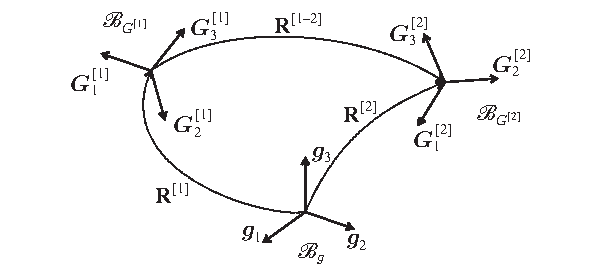
\includegraphics{Dodatki/slike/KompozitumRotacij}
\bicaption[fig: Kompozitum rotacij]{}{
Kompozitum rotacij.
}{Figure}{
Composition of rotations.}
\addfiguretolof{Composition of rotations.}
\end{center}
\end{figure}
%
%
Vektorje, izra?ene v posameznih bazah, lahko z rotacijskimi matrikami 
izrazimo v drugih bazah. Tako lahko na primer z rotacijsko matriko 
$\bm{R}^{\left[1-2\right]}$ 
poljuben vektor baze $\mathcal{B}_{G^{\left[ 2\right] }}$ izrazimo v bazi 
$\mathcal{B}_{G^{\left[ 1\right] }}$ kot 
$\bs{G}_{i}^{\left[2\right]} = \bm{R}^{\left[1-2\right]} 
\bs{G}_{i}^{\left[1\right]}$. Podobno 
bazni vektor $\bs{G}_{i}^{\left[1\right]}$ 
zapi?emo kot zavrten vektor $\bs{g}_{i}$ baze $\mathcal{B}_{g}$:
$\bs{G}_{i}^{\left[1\right]} = \bm{R}^{\left[1\right]} \bs{g}_{i}$.

?e zgornja zapisa zdru?imo, dobimo zvezo med baznimi vektorji baz 
$\mathcal{B}_{g}$ in $\mathcal{B}_{G^{\left[ 2\right] }}$:
\begin{equation*}
\bs{G}_{i}^{\left[2\right]} = \bm{R}^{\left[1-2\right]} \bm{R}^{\left[1\right]} \bs{g}_{i}.
\end{equation*}
%
Rotacijska matrika $\bm{R}^{\left[2\right]}$ je torej
\begin{equation}
\bm{R}^{\left[2\right]} = \bm{R}^{\left[1-2\right]} \bm{R}^{\left[1\right]}.
\label{eq: kompozitum rotacij}
\end{equation}
%
Za zdru?itev dveh rotaciji v eno samo moramo torej uporabiti 
operacijo mno?enja in ne se?tevanja, kar poudarimo tudi z izrazom 
`kompozitum rotacij'. Pokazali smo ?e, da ima rotacijska matrika 
enak komponentni zapis v bazah, med katerima slika, zato lahko tudi 
kompozitum rotacij v izrazu \eqref{eq: kompozitum rotacij} 
zapi?emo v eni od obeh baz:

\begin{equation*}
\bm{R}_{g}^{\left[2\right]} = \bm{R}_{g}^{\left[1-2\right]} \bm{R}_{g}^{\left[1\right]}
= \bm{R}_{G^{\left[2\right]}}^{\left[2\right]} = 
\bm{R}_{G^{\left[2\right]}}^{\left[1-2\right]} \bm{R}_{G^{\left[2\right]}}^{\left[1\right]}.
\end{equation*}

V primeru, da imamo rotacijsko matriko $\bm{R}^{\left[1-2\right]}$ 
izra?eno glede na bazo 
$\mathcal{B}_{G^{\left[ 1\right] }}$, dobi kompozitum rotacij 
\eqref{eq: kompozitum rotacij} z uporabo pravila \eqref{eq: transformacija matrike} 
naslednjo obliko:
\begin{equation}
\bm{R}_{g}^{\left[2\right]} = \bm{R}_{g}^{\left[1\right]} 
\bm{R}_{G^{\left[1\right]}}^{\left[1-2\right]}
\bm{R}_{g}^{\left[1\right]T} \bm{R}_{g}^{\left[1\right]}
 = \bm{R}_{g}^{\left[1\right]} 
 \bm{R}_{G^{\left[1\right]}}^{\left[1-2\right]}.
\label{eq: kompozitum rotacij v lokalni bazi}
\end{equation}
Pomembno je torej, da smo pri komponiranju rotacij pozorni na to, 
v katerih bazah so posamezne rotacijske matrike zapisane. Od tega je 
namre? odvisen vrstni red mno?enja rotacijskih matrik.


%-----------------------------------------------------------
\section{Parametrizacija rotacij}
\label{sec: Parametrizacija rotacij}
%-----------------------------------------------------------
Rotacijska matrika ima devet komponent, od katerih pa so  
zaradi lastnosti \eqref{eq: rotacijska matrika je ortogonalna} 
le tri med seboj neodvisne. 
Za izpeljavo ena?b nosilca je zato ugodneje uporabiti druga?en 
zapis rotacij. Med najpogosteje uporabljenimi je 
rotacijski vektor $\bs{\vartheta}$, ki je dolo?en s smerjo 
$\bs{n}$ in velikostjo rotacije $\vartheta$:
\begin{equation}
\bs{\vartheta} = \vartheta \bs{n}.
\end{equation}
%
?e vpeljemo anitisimetri?no matriko $\bm{S}\left(\bs{u} \right)$, 
ki pripada poljubnemu vektorju $\bs{u}$:
\begin{equation}
\bm{S}\left(\bs{u} \right) = 
\left[ 
\begin{array}{ccc}
0	 	 & -u_{3}	 & u_{2} \\
u_{3}	 & 0		 & -u_{1} \\
-u_{2}	 & u_{1}	 & 0 
\end{array}
\right] = -\bm{S}\left(\bs{u} \right)^{T},
\end{equation}
lahko rotacijsko matriko, parametrizirano z rotacijskim 
vektorjem, izrazimo z Rodriguesovo formulo \cite{Argyris1982,ZupanPhd2003}
\begin{equation}
\bm{R}\left(\bs{\vartheta} \right) = 
\bm{I}+\dfrac{\sin \vartheta}{\vartheta} 
\bm{S} \left( \bs{\vartheta}\right) +
\dfrac{1-\cos \vartheta}{\vartheta^2}
\bm{S}^2 \left( \bs{\vartheta}\right).
\label{eq: Rodriguesova formula}
\end{equation}
%
Pri tem je $\bm{I}$ identiteta in 
$\vartheta = \left\| \bs{\vartheta}\right\| =
\sqrt{\vartheta_{1}^{2} + \vartheta_{2}^{2} + 
\vartheta_{3}^{2}}$. 

Ob znani rotacijski matriki lahko njej pripadajo?i rotacijski vektor 
izra?unamo s Spurrierovim algoritmom \cite{Spurrier1978}. 
Ker je $\bs{\vartheta}$ lastni vektor matrike $\bm{R}$, velja
$\bs{\vartheta}_{g} = \bm{R}\bs{\vartheta}_{G} = \bs{\vartheta}_{G}$.

Za izpeljavo ena?b v okviru tega dela je smiselno vpeljati tudi 
operator $\bm{A}$, ki antisimetri?ni matriki priredi njen 
osni vektor $\bs{u}$
\begin{equation}
\bm{A}\left( \bm{S}\left( \bs{u}\right) \right) = \bs{u},
\end{equation}
%
in pripraviti nekaj zvez med antisimetri?nimi matrikami 
in njihovimi osnimi vektorji, ki izpeljave ena?b poenostavijo. 
Naj bosta $\bs{u}$ in $\bs{v}$ poljubna vektorja. Potem velja:
\begin{align}
\left(\bs{u} \cdot \bs{v}\right) 
\bm{S}\left(\bs{u}\right) &= 
-\bm{S}\left(\bs{u}\right) \bm{S}\left(\bs{v}\right) 
\bm{S}\left(\bs{u}\right)
\label{eq: lastnost antisimetricnih matrik 1}
\\
\bm{S}\left(\bs{u}\right)\bm{S}\left(\bs{v}\right)-
\bm{S}\left(\bs{v}\right)\bm{S}\left(\bs{u}\right) &=
\bm{S}\left( \bm{S}\left(\bs{u}\right) \bs{v} \right)
\label{eq: lastnost antisimetricnih matrik 2}
\\
\left(\bs{u} \cdot \bs{v}\right) \bm{S}\left(\bs{u}\right)
- \left(\bs{u} \cdot \bs{u}\right)\bm{S}\left(\bs{v}\right) &=
\bm{S}\left(\bm{S}^{2}\left(\bs{u}\right)\bs{v}\right).
\label{eq: lastnost antisimetricnih matrik 3}
\end{align}
%
Z antisimetri?nim operatorjem lahko nadomestimo tudi vektorski 
produkt dveh poljubnih vektorjev $\bs{u}$ in $\bs{v}$:
\begin{equation}
\bs{u}\times\bs{v} = \bm{S}\left(\bs{u}\right)\bs{v} = 
- \bm{S}\left(\bs{v}\right)\bs{u}.
\label{eq: vektorski produkt izrazen z antisimetricno matriko}
\end{equation}
%
Iz identitete 
$\bm{S}\left( \bs{u}\right) = \bm{R}^{T}\bm{S}\left( \bs{v}\right) \bm{R}$ sledi
\begin{equation}
\bs{u} = \bm{R}^{T} \bs{v}.
\label{eq: relacija u v}
\end{equation}


%-----------------------------------------------------------
\section{Variacija rotacijske matrike, parametrizirane 
			z rotacijskim vektorjem}
\label{sec: Variacija rot vektor}
%-----------------------------------------------------------
Variacijo rotacijskega operatorja lahko v na�em primeru izra?unamo s smernim odvodom. 
Pri tem upo?tevamo 
definicijo smernega odvoda, ki pravi, da je smerni odvod rotacije limita z 		
$\epsilon\delta\bs{\vartheta}$ povzro?ene spremembe operatorja $\bm{R}$, ko gre 
$\epsilon$ proti ni?. Rotacija, ki pripada spremembi 
rotacijskega vektorja $\epsilon\delta\bs{\vartheta}$, je enaka
$\bm{R(\epsilon\delta\bs{\vartheta})}$, skupna rotacija pa je kompozitum trenutne 
rotacije in njene spremembe:
$\bm{R(\epsilon\delta\bs{\vartheta})}\bm{R(\vartheta)}$.
%

Smerni odvod rotacijske matrike torej izra?unamo kot
\begin{equation*}
\delta \bm{R}\left(\bs{\vartheta} \right) = 
\dfrac{d}{d\epsilon}\bigg|_{\epsilon=0} 
\bm{R}\left( \epsilon\delta \bs{\vartheta} \right) 
\bm{R}\left( \bs{\vartheta}\right) .
\end{equation*}
%
$\bm{R}\left( \epsilon\delta\vartheta \right)$ zapi?emo z 
Rodriguesovo formulo \eqref{eq: Rodriguesova formula},
 odvajamo po $\epsilon$, izvrednotimo 
pri $\epsilon = 0$ in dobimo:
\begin{equation}
\delta \bm{R}\left(\bs{\vartheta} \right) =
\bm{S}\left( \delta \bs{\vartheta}\right) 
\bm{R}\left(\bs{\vartheta} \right) .
\end{equation}
%
Sprememba rotacije pa je lahko dolo?ena tudi kot komponiranje z 
desne $\bm{R}\left(\bs{\vartheta}_{g}\right) 
\bm{R}\left(\epsilon\delta\bs{\vartheta}_{G}\right)$ 
(v tem zapisu smo z indeksom $g$ poudarili, da gre za bazo $\mathcal{B}_{g}$, 
v nadaljevanju izpeljave pa $g$ pri $\vartheta$ opu??amo).
Sledi
\begin{equation}
\delta \bm{R}\left(\bs{\vartheta} \right) =
\bm{R}\left(\bs{\vartheta} \right)
\bm{S}\left( \delta \bs{\vartheta}_{G}\right) . 
\label{eq: odvod rotacije z desne}
\end{equation}
%
Ker morata biti variaciji obeh izrazov enaki, velja
\begin{equation}
\bm{S}\left( \delta \bs{\vartheta}_{G}\right) = 
\bm{R}^{T} \bm{S}\left( \delta \bs{\vartheta}_{g}\right) \bm{R}.
\end{equation}
%
Od tod in iz ena�be \eqref{eq: relacija u v} je potem
\begin{equation}
\delta \bs{\vartheta}_{G} = \bm{R}^{T} \delta \bs{\vartheta}_{g}.
\end{equation}

V ena?bah nosilca variacija rotacijske matrike ve?krat deluje 
na vektorju. Ob upo?tevanju ena?be 
\eqref{eq: vektorski produkt izrazen z antisimetricno matriko} izpeljemo
\begin{equation}
\delta \bm{R}\left( \bs{\vartheta} \right) \bs{u} = 
\bm{S} \left( \delta \bs{\vartheta} \right) 
\bm{R}\left( \bs{\vartheta} \right) \bs{u} = 
\delta \bs{\vartheta} \times \bm{R}\left( \bs{\vartheta} \right) \bs{u} = 
- \bm{R}\left( \bs{\vartheta} \right) \bs{u} \times \delta \bs{\vartheta} = 
- \bm{S} \left( \bm{R}\left( \bs{\vartheta} \right) \bs{u}\right) 
\delta \bs{\vartheta}. 
\label{eq: variacija rotacije na vektorju neaditivno}
\end{equation}
%
Variacijo rotacijske matrike, ki deluje na poljubnem vektorju $\bs{u}$, 
lahko torej izrazimo z variacijo rotacijskega vektorja.


%-----------------------------------------------------------
\section{Variacija rotacijske matrike, parametrizirane 
				z aditivnim rotacijskim vektorjem}
\label{sec: Variacija adititvni rot vektor}
%-----------------------------------------------------------
V primeru meh?anja materiala so glede na izbrani opis 
deformacij \eqref{eq: deformacijski nastavek za game} in 
\eqref{eq: deformacijski nastavek za kape} funkcije kinemati?nih koli?in 
izra?ene z zveznim in nezveznim delom. Slednji je zapisan v telesni bazi prostora, zato se 
sre?amo z rotacijskimi matrikami, parametriziranimi z rotacijskim vektorjem, ki je zapisan 
v telesni bazi prostora: $\bm{R} \left( \bs{\vartheta}_G \right)$. Njihove spremembe 
dolo?amo s komponiranjem z desne, smerni odvod pa z izrazom
\begin{equation}
\delta \bm{R}\left(\bs{\vartheta}_G \right) = 
\dfrac{d}{d\epsilon}\bigg|_{\epsilon=0} 
\bm{R}\left( \bs{\vartheta}_G \right)
\bm{R}\left( \epsilon\delta \bs{\vartheta}_G \right).
\end{equation}

%
Rotacijo $\bm{R}\left( \epsilon\delta \bs{\vartheta}_G \right)$, ki pripada spremembi 
rotacijskega vektorja $\epsilon\delta \bs{\vartheta}_G$, zapi?emo z Rodriguesovo formulo 
\eqref{eq: Rodriguesova formula}, odvajamo po $\epsilon$ in izvrednotimo pri $\epsilon=0$. 
Tako dobimo:
\begin{equation}
\delta \bm{R}\left(\bs{\vartheta}_G \right) = 
\bm{R}\left( \bs{\vartheta}_G \right)
\bm{S}\left( \delta \bs{\vartheta}_G \right).
\label{eq: variacija rotacije pri komponiranju z desne}
\end{equation}

Spremenjeno rotacijsko matriko pa lahko opi?emo tudi tako, 
da rotacijskemu vektorju spremembo kar pri?tejemo: 
$\bm{R}\left(\bs{\vartheta}_{G} + 
\epsilon\delta\bs{\vartheta}_{G}^{A} \right)$. Pri tem je 
$\delta\bs{\vartheta}_{G}^{A}$ tako imenovani `aditivni' 
rotacijski vektor, dolo?imo pa ga tako, da velja
\begin{equation}
\delta \bm{R}\left(\bs{\vartheta}_{G}\right)  = 
\dfrac{d}{d\epsilon}\bigg|_{\epsilon=0} 
\bm{R}\left(\bs{\vartheta}_{G} + 
\epsilon\delta\bs{\vartheta}_{G}^{A} \right).
\end{equation}
%
$\bm{R}\left(\bs{\vartheta}_{G} + 
\epsilon\delta\bs{\vartheta}_{G}^{A} \right)$ 
zapi?emo z Rodriguesovo formulo \eqref{eq: Rodriguesova formula}, 
odvajamo po $\epsilon$ in izvrednotimo pri $\epsilon=0$:
\begin{align}
\delta \bm{R}\left(\bs{\vartheta}_{G}\right)  = & \,
\dfrac{\sin \vartheta}{\vartheta}\bm{S}\left( \delta\bs{\vartheta}_{G}^{A}\right) 
+ \dfrac{1-\cos\vartheta}{\vartheta^2}
\left( 
\bm{S}\left( \delta\bs{\vartheta}_{G}^{A}\right) \bm{S}\left( \bs{\vartheta}_{G}\right)
+ \bm{S}\left( \bs{\vartheta}_{G}\right) \bm{S}\left( \delta\bs{\vartheta}_{G}^{A}\right)
\right) \notag\\
&+ \dfrac{\vartheta \cos \vartheta - \sin \vartheta}{\vartheta^3}
\left( 
\bs{\vartheta}_{G} \cdot \delta\bs{\vartheta}_{G}^{A}
\right) \bm{S}\left( \bs{\vartheta}_{G} \right)  \notag \\
&+ \dfrac{\vartheta \sin \vartheta - 2\left( 1-\cos \vartheta\right) }{\vartheta^4}
\left( 
\bs{\vartheta}_{G} \cdot \delta\bs{\vartheta}_{G}^{A}
\right) \bm{S}^2\left( \bs{\vartheta}_{G} \right).
\label{eq: variacija rotacijske matrike aditivno}
\end{align}
%
Za variacijo rotacijske matrike v smislu aditivnega rotacijskega vektorja 
lahko z upo?tevanjem lastnosti \eqref{eq: rotacijska matrika je ortogonalna} 
poka?emo, da je produkt 
$\delta \bm{R}\bm{R}^{T}$ antisimetri?na matrika
\begin{equation*}
\bm{R}\bm{R}^{T} = \bm{I} \qquad \Rightarrow \qquad
\delta \bm{R}\bm{R}^{T} + \bm{R} \delta \bm{R}^{T} = 0 
\qquad \Rightarrow \qquad
\delta \bm{R}\bm{R}^{T} =- \bm{R} \delta \bm{R}^{T} = 
- \left( \delta \bm{R}\bm{R}^{T}\right) ^{T} .
\end{equation*}
%
?e sedaj izraz \eqref{eq: variacija rotacijske matrike aditivno} z desne 
pomno?imo z $\bm{R}^{T}\left( \bs{\vartheta}_{G}\right) $ in upo?tevamo 
anitisimetri?nost produkta $\delta \bm{R}\bm{R}^{T}$, 
dobimo po kon?anem urejanju
\begin{equation}
\delta \bm{R}\left(\bs{\vartheta}_{G}\right) 
\bm{R}^{T}\left(\bs{\vartheta}_{G}\right) = 
\bm{S} 
\left(
\delta \bs{\vartheta}_{G}^{A}+ 
\dfrac{1-\cos\vartheta}{\vartheta^2}\bm{S}\left( \bs{\vartheta}_{G} \right)
\delta \bs{\vartheta}_{G}^{A} + 
\dfrac{\vartheta-\sin\vartheta}{\vartheta^3}
\bm{S}^2\left( \bs{\vartheta}_{G} \right)\delta \bs{\vartheta}_{G}^{A}
\right) ,
\end{equation}
pri ?emer lahko na desni strani izraza prepoznamo produkt transformacijske 
matrike $\bm{T}\left( \bs{\vartheta}_{G}\right) $ 
\begin{equation}
\bm{T}\left( \bs{\vartheta}\right) = 
\bm{I} + \dfrac{1-\cos\vartheta}{\vartheta^2} \bm{S}\left( \bs{\vartheta}\right) + 
\dfrac{\vartheta-\sin\vartheta}{\vartheta^3} \bm{S}^2\left( \bs{\vartheta}\right)
\label{eq: transformacijska matrika}
\end{equation}
%
in aditivne variacije 
$\delta \bs{\vartheta}_{G}^{A}$. Potem je
\begin{equation}
\delta \bm{R}\left(\bs{\vartheta}_{G}\right) 
\bm{R}^{T}\left(\bs{\vartheta}_{G}\right) = 
\bm{S} 
\left(
\bm{T}\left( \bs{\vartheta}_{G}\right)
\delta \bs{\vartheta}_{G}^{A}
\right) .
\label{eq: variacija v smislu aditivnega vektorja}
\end{equation}
%
Izraz \eqref{eq: variacija v smislu aditivnega vektorja} lahko sedaj 
primerjamo z izrazom \eqref{eq: variacija rotacije pri komponiranju z desne}, ki ga z desne 
pomno?imo z $\bm{R}^{T}\left( \bs{\vartheta}_{G}\right) $. Tako dobimo
povezavo med aditivno variacijo $\delta \bs{\vartheta}_{G}^{A}$ in
multiplikativno variacijo $\delta \bs{\vartheta}_{G}$:
\begin{equation}
\delta \bs{\vartheta}_{G} = 
\bm{R}^{T}\left(\bs{\vartheta}_{G}\right) 
\bm{T}\left( \bs{\vartheta}_{G}\right)
\delta \bs{\vartheta}_{G}^{A} = 
\bm{T}^{T}\left( \bs{\vartheta}_{G}\right)
\delta \bs{\vartheta}_{G}^{A}.
\label{eq: aditivna - multiplikativna variacija}
\end{equation}
%
Pri tem smo upo?tevali zvezo $\bm{R}^{T} \bm{T} = \bm{T}^{T}$.

Tudi variacijo rotacijske matrike v smislu aditivnega rotacijskega vektorja 
$\delta \bm{R}\left( \bs{\vartheta}_{G}\right) $, ki deluje na 
poljubnem vektorju $\bs{u}$, je zaradi re?evanja ena?b koristno 
izraziti z variacijo aditivnega rotacijskega vektorja. 
Izraz \eqref{eq: variacija rotacije pri komponiranju z desne} najprej 
pomno?imo z $\bs{u}$, upo?tevamo 
\eqref{eq: aditivna - multiplikativna v
\begin{align}
\delta \bm{R} \left( \bs{\vartheta}_{G}\right) \bs{u} &= 
\bm{R} \left( \bs{\vartheta}_{G}\right) 
\bm{S} \left( \delta \bs{\vartheta}_{G}\right) \bs{u} \notag \\
&= -\bm{R} \left( \bs{\vartheta}_{G}\right)
\bm{S} \left( \bs{u}\right) \delta \bs{\vartheta}_{G} \notag \\
&= -\bm{R} \left( \bs{\vartheta}_{G}\right)
\bm{S} \left( \bs{u}\right)\bm{T}^{T}\left( \bs{\vartheta}_{G}\right)
\delta \bs{\vartheta}_{G}^{A}.
\label{eq: variacija rotacije na vektorju aditivno}
\end{align}

%\include{Dodatki/DodatekB}
%\include{Dodatki/DodatekC}
%\include{Dodatki/DodatekD}
%\include{Dodatki/DodatekE}


\end{document}

